\documentclass{article}
\usepackage{graphicx}
\usepackage{hyperref}
\usepackage[a4paper, margin=1in]{geometry}
\usepackage{breakcites}
\usepackage{subcaption}
\usepackage{multicol}
\usepackage{booktabs}
\usepackage{longtable}

\begin{document}

\title{Mapping Africa's Natural Safety Nets: Where Should Conservation Efforts Be Targeted to Sustain Ecosystem Services for Climate Change Resilience?}

\author{
	Cooper, Matthew\\
	%Zvoleff, Alex \\
	%Sanders, Austin \\
}

%Add new pub: https://www.tandfonline.com/doi/abs/10.1080/02255189.2020.1781600

\maketitle
\begin{abstract}

In Africa, where millions of households depend on rainfed agriculture to produce food for their own consumption, climate change is a major threat to food security.  A large literature suggests that natural areas can be an asset in the face of climate change by shielding cropland from the effects of droughts and heat waves, while also providing wild foods when yields are low.  However, much of the work focusing on the "safety net" provided by natural and uncultivated land cover types has been conducted in highly localized and site-specific case studies which often rely on hypothetical or retrospective analyses.  Thus, there has been little empirical and spatially explicit work on which areas provide the most benefit to local food security.  In this study, we combine data on nutrition outcomes from 221,225 children in agrarian communities across 32 African countries with historical observations of land cover and climate shocks to test the safety net hypothesis and to map the areas that have historically played the greatest role in supporting nutrition outcomes during shocks.  These results will help conservationists to target areas providing the most benefit to local food security and nutrition and improve future conservation planning efforts.

\end{abstract}

\section{Introduction}

Currently, an estimated 58.8 million African children, representing nearly one third of the continent's under-5 population, suffer from chronic undernutrition \cite{unicef2019}.  While progress has been made in the past several decades to improve nutrition and food security outcomes, climate change threatens to stall or even reverse current trends \cite{FAO2018}.  As climate change continues, the frequency and intensity of meteorological extremes will affect food production, ultimately harming food security and nutrition for many vulnerable communities.  No continent is more vulnerable to these changes than sub-Saharan Africa, where an estimated 95\% of agriculture is rainfed \cite{Wani2009} and about 65\% of households  produce food for their own consumption \cite{Runge2004}.

One factor that can play a major role in fostering food systems that are resilient to climate shocks is the presence of ecosystem services provided by forests, savannas, and other natural, uncultivated land use types.  Uncultivated areas provide a suite of regulating services that can buffer agricultural yields from the effects of shocks.  For example, natural vegetation can provide shade and cooler temperatures during heat waves, absorb water and protect against erosion during floods, as well as retain soil moisture during droughts.  Furthermore, natural areas can provide habitat for pollinators and species that regulate pest outbreaks.  Beyond regulating services, natural, uncultivated land provides provisioning services in the form of wild foods and other inedible Non-Timber Forest Products that can support local incomes and food security when agricultural output is low.

While a great deal of literature has focused on the benefit that ecosystem services can provide, much of this work has relied on studies that are site specific.  For example, detailed work conducted in case studies across Africa have found instances of ecosystem services improving child nutrition \cite{Golden2011}, regulating crop pests \cite{Girma2000}, improving yields through pollination \cite{Gemmill-Herren2008, Munyuli2012}, and improving soil nutrient quality \cite{Sileshi2012, Boffa2000, Siriri2009}.  Some work that is particularly relevant to climate resilience has found that natural land cover can improve soil water storage \cite{Siriri2013, Lott2009}, but nevertheless few empirical studies have observed how ecosystem services affect human outcomes during climate shocks.  Rather, most studies that focus on ecosystems as a form of climate resilience use surveys that ask respondents if they would rely on ecosystem services in the event of a hypothetical shock \cite{Robledo2012}, with some studies indicating that many people do not think of ecosystem services as an asset that they would rely on during a shock \cite{Wunder2014}.

Building on all these case studies, a growing body of work has drawn on Demographic and Health Surveys from across Africa and the developing world to assess whether the benefits provided by various ecosystem services can be observed at scale.  This work has shown that forest cover is associated with improved dietary diversity \cite{Ickowitz2014, Rasolofoson2018}, that forested watersheds are associated with less diarrheal disease \cite{Herrera2017}, and that protected areas are associated with a number of positive benefits \cite{naidoo2019evaluating}.  Our work builds on these studies by examining the benefit that natural, uncultivated land cover types provide to nutrition outcomes specifically during droughts.  Furthermore, this study goes beyond testing for an association across the entire dataset, but also examines how the relationship between climate shocks, natural land cover, and rainfall varies across Agro-Ecological Zones (AEZs) to identify areas where natural land cover provides the greatest benefit to child nutrition outcomes.

While a large body of research attests to the fact that ecosystem services play a large role in food production and nutrition, especially for smallholder farmers, comparatively little work in the field of environmental conservation has been conducted to identify areas where conservation interventions could lead to improved food security and nutrition outcomes.  This is in spite of the fact that the practice of conservation relies heavily on mapping for priority setting - for example, mapping ecosystem services such as carbon sequestration and storage or water provision as well as mapping biodiversity hot spots.  Thus, mapping which natural areas contribute the most to climate-resilient nutrition systems could further catalyze conservation investment, as well as identify locations where conservation interventions could lead to synergies between Sustainable Development Goals (SDGs) related to environmental conservation (13 \& 15) and human well-being (1 \& 2).

\section{Theoretical Framework}

\subsection{Land Cover and Ecosystem Services}
The ecosystem services provided by nature are highly varied and operate across different spatial scales.  They are typically classified into provisioning, supporting, regulating, and cultural services \cite{Martinez-Harms2012}, although other typologies exist \cite{Fisher2008}.  A common approach for mapping ecosystem services is to focus on land cover types, especially when primary data is unavailable \cite{Martinez-Harms2012}.  One approach is to analyze each landcover type as providing a ``bundle" of associated ecosystem services \cite{Raudsepp-Hearne2010}.  Thus, in an African context, cultivated land provides food crops as a service, grasslands providing grazing for livestock as well as habitat for pollinators and pest regulation services, while forests provide a variety of wild foods, soil formation, water quality regulation, and non-timber forest products.  This framework is especially useful for analyzing trade-offs: as natural vegetation is cleared to make room for crop production, the increase in food crops necessitates a decrease in habitat for pollinators and wild food species, as well as the regulating services provided by uncultivated land.  Conversely, as agricultural land is abandoned, it stops providing food crops but becomes available again for timber production, water quality regulation and erosion protection, etc.  Finally, previous work has shown that natural, uncultivated land is one of the best geographic predictors of whether households in Africa report collecting both wild foods as well as other provisioning ecosystem services \cite{Cooper2018a}.

\subsection{Uncultivated Land and Commons}
The regulating and supporting services provided by uncultivated land, such as soil formation, pollination, and water retention are, by their very nature, beneficial across boundaries of property and ownership.  However, in cases when land is privately held, provisioning services such as food crops or timber only provide benefits to landowners, who reserve the right to collect these goods.  

In Africa, uncultivated land is often held as a commons, providing resources multiple members of a community rather than just one landowning household, although specific practices of land tenure, ownership, access rights, and communal domain vary widely across cultural contexts \cite{Wily2008}.  This means that not only regulating and supporting services but even provisioning services such as wild foods and fuelwood provided by uncultivated land are available to many members of a community.  Thus, these areas are especially critical for the poorest members of communities, and these commons are often framed as ``possibly the only capital asset of the poor" \cite{Wily2008}.  Furthermore, empirical research has shown that provisioning services provided by such areas are critical for the livelihoods of women, migrants, and other marginalized groups in rural Africa \cite{Coulibaly-Lingani2009, Pouliot2013}.

Thus, as cropland expands into previously uncultivated areas in Africa due to pressures of both population growth and agricultural commodification \cite{Rudel2013, Laurance2014}, commons and the services they provide for communities and the poor are becoming increasingly depleted.  The conversion of communal land to privately held, cultivated land often happens with no benefit to marginalized community members because communally held land and commons are not well-recognized or protected by African legal systems \cite{Wily2011}.

\subsection{Sustainable Livelihoods Approach}
One framework for assessing how rural agrarian peoples respond to shocks is the Sustainable Livelihoods Approach (SLA), which emerged in the 1990's as a way to understand how impoverished agricultural people maximize their access to various capitals in order to ensure the sustainability and resilience of their livelihoods in the face of risks and challenges \cite{Scoones1998a, Ellis1998, Bebbington1999}.  One defining feature of SLA is that it views people as agents working actively to maximize their overall well-being rather than just passive victims of a specific political or environmental context \cite{Adato2002}.  Scoones originally identified four types of capital that communities utilize to further their livelihood goals: natural capital, financial capital, human capital, and social capital, although there are many other types of capital that communities use as well \cite{Scoones1998a}.  For this analysis, we view drought vulnerability as determined, in part, by the tradeoff in agricultural capital provided by cultivated areas and natural capital provided by uncultivated areas.

\section{Data Sources}

\subsection{Nutrition Data}

For this analysis, we use data from Demographic and Health Surveys (DHS) from throughout Africa.  The DHS is often considered the ``gold standard'' of data on health and nutrition from developing countries and is often used in environmental health studies, because the GPS coordinates associated with each DHS site make it possible to infer the environmental context at the time and location of the survey \cite{Brown2014}.  We utilize all surveys from sub-Saharan Africa that meet the following criteria: (1) they have geolocated coordinates, to facilitate the extraction of climate conditions and local land cover at the site of each DHS site, (2) they have data on child nutrition outcomes, and (3) they have data on relevant household and individual co-variates of malnutrition.

As our metric of child nutrition, we use Height-for-Age Z-Scores (HAZ Scores).  This is an indicator of stunting, a consequence of long-term malnutrition, and has been collected in the majority of DHS surveys for decades.  HAZ Scores are derived by comparing the height of a child under five years of age to the distribution of heights of well-nourished children of the same age and gender, and then deriving a Z-score.  While natural variation in human height makes it impossible to diagnose any one individual as stunted \cite{Perumal2018}, stunting can be defined at the population level as the percentage of a population with an HAZ score less than -2, and severe stunting is the percentage of a population with an HAZ score less than -3.  While human populations do vary in potential attainable height, for children under 5, differences in height are mostly explained by environmental and dietary conditions \cite{Habicht1974}.

\subsection{Drought Data}
For our data on drought, we use precipitation data from the Climate Hazards Infrared Precipitation with Stations (CHIRPS) dataset \cite{Funk2015} and temperature data a land surface re-analysis model \cite{Sheffield2006}.  Because direct observations of long-term climate conditions in Africa are scarce, both of these datasets rely on remote sensing as well as modeling to infer meteorological conditions across space.

Using monthly estimates of precipitation as well as average daily monthly maximum and minimum temperatures, we calculate the monthly water balance using the Hargreaves method \cite{Hargreaves1982} and then derive the 24-month Standardized Precipitation-Evapotranspiration Index (SPEI) \cite{Begueria2014}.  This metric compares the water balance over the previous 24 months and compares it to long-term trends in that location, deriving an index that can be interpreted like a Z-Score.  In previous studies of precipitation anomalies and child malnutrition, the SPEI calculated for the 24 months before a survey was the best predictor of child health outcomes \cite{Cooper2019Mapping}.  Because the SPEI accounts for both precipitation anomalies as well as water lost through heat-induced evapotranspiration, it can characterize both meteorological and hydrological droughts, both of which are expected to become more common under climate change \cite{Dai2013}.

While drought has a strong and clear impact on children's nutrition status in many parts of Africa, excessive rainfall can also affect health outcomes \cite{Cooper2019Mapping}.  To focus only on the effects of drought relative to normal periods, we exclude from our analysis children observed during relatively high levels of rainfall (SPEI \textgreater 1).

\subsection{Land Cover}
For data on land cover near a DHS site, we use a dataset created by the European Space Agency Climate Change Initiative \cite{Defourny2017}, which is available annually for the years 1992 to 2015 at a 300m resolution for 22 distinct land cover classes.  For uncultivated land providing regulating, supporting, and communal provisioning ecosystem services, we use all forms of tree, shrub and herbaceous cover, as well as shrubland, grassland, and water bodies.  Additionally, for mosaic land cover types with both cropland and natural vegetation, we counted each pixel as cultivated if it contained more than 50\% cropland and uncultivated if it contained less than 50\% cropland.  Finally, we do not count urban, bare, or permanent snow and ice areas as uncultivated land, as they do not provide most of the local ecosystem services that uncultivated land cover types do.

As our metric for the availability of ecosystem services, we determine the fraction of land within 15 km of each DHS site that was uncultivated at the time of the survey.  We use a 15 km radius for three reasons.  For one, DHS sites are spatially distorted to preserve respondent anonymity, with 99\% of sites displaced by up to 5 km and 1\% of sites displaces by up to 10 km \cite{Grace2012}.  Thus, a 15 km radius more accurately captures landscape-scale land cover characteristics, because the land cover in the immediate vicinity of a community can't be known.  We also focus on a 15 km, landscape-scale area because many ecosystem services flow over large scales, especially abiotic resources that move through space, such as water, as well as ecosystem services from animals, such as bushmeat and pollination \cite{Lopez-Hoffman2010}.  Finally, many individuals will travel significant distances to farm and to collect resources, especially in swidden cropland systems as well as when resources are scarce \cite{Felardo2016, Arku2010}.

Having derived nearby land-cover categories for each DHS site, we exclude sites from our analysis that have greater than 1\% of nearby land cover as urban or greater than 5\% of nearby land cover as water.  This is to ensure that we are basing our analysis only on rural, agrarian households that are largely dependent on rainfed agricultural and ecosystem services from non-agricultural areas.  Excluding DHS sites that were either observed during a significantly wet period (SPEI \textgreater 1) or in urban or coastal areas, yields a dataset of 221,885 observations, or 59.6\% of the original 372,197 observations.

\subsection{Agro-Ecological Zones}
Because both farm systems and ecosystem services vary according to local biophysical variables, especially temperature, precipitation and elevation, we analyze the effect of ecosystem services in providing drought resilience at the scale of Agro-Ecological Zones (AEZs).  Using the FAO methodology \cite{Fischer2006} AEZs are defined by elevation and length of growing period, where the growing period is defined as days where precipitation plus moisture stored in the soil exceeds half of potential evapotranspiration \cite{Fischer2006}.  In other parts of the world, temperature is an important factor in determining AEZ, but as nearly all of Africa is warm, it is not an important determinant in this analysis.  In cases where there are ample observations (Savanna and Sub-Forest), we disaggregate each zone into roughly contiguous northern and southern hemisphere zones.  Conversely, in the case of arid zones, where there was fewer observations we aggregated across across the entire continent to create one discontinuous zone, assuming that the relationships between drought, ecosystem services, and nutrition outcomes are comparable across all of arid Africa.  In the end, each zone in our analysis had over 10,000 child nutrition observations from multiple countries and surveys (See Table \ref{table:AEZtab}).

Briefly, here is an overview of each AEZ in our analysis:

\begin{itemize}
	\item \textbf{Arid}: This AEZ includes all parts of Africa with a growing period of less than 70 days a year throughout the Sahel and Sahara, the Horn of Africa as well as the Kalahari desert.  Livelihood systems in arid parts of Africa are often completely pastoral, although in some cases arid-adapted crops like Sorghum and Millet are grown.  Population is typically quite sparse.
	\item \textbf{Forest}: This AEZ includes all areas over 270 days of growing period in a year.  Forests are primarily found in central Africa, but are also in mountainous and coastal parts of West Africa, in Liberia and Sierra Leone, as well is in coast Southeast Africa, in Mozambique and Madagascar.  Farming activities in these areas are based around crops like rice and cassava, as well as commodity tree crops like rubber and palm oil.  Populations in agricultural areas are typically sparse, although greater population density can be found along coasts and rivers.
	\item \textbf{Highlands}: For highlands, we included all areas at greater than 1200m of elevation, irrespective of growing period.  This included much of the highlands of Ethiopia, Eastern and Southern Africa, as well as Lesotho.  Livelihood systems in mountainous regions are primarily crop-based, although the particular crops vary, with Teff and Wheat being prevalent in Ethiopia and crops like Potatoes, Maize and Bananas being more prevalent in Southern and Eastern Africa.  Cash crops include Coffee and Tea.  In much of the highlands of Africa population and agriculture are quite dense.
	\item \textbf{Northern Savanna}:  The Northern African Savanna, typically called Sahelian Savanna is characterized by 70-180 day growing seasons and extends from Senegal to the Sudan.  Crops include maize, groundnuts, millet, and sesame, and cattle production is high.  Population densities vary substantially from the dense Hausalands of northern Nigeria to more remote parts of Chad, but generally high.
	\item \textbf{Southern Savanna}: Also characterized by 70-180 day growing seasons, Southern African Savanna occupies a swath of lowlands from southern Kenya, through Tanzania and Zambia to the Victoria falls region of Southern Africa.  Agriculture includes maize and cattle.  Population densities vary but are generally more sparse than the savannas of Northern Africa, with significant amounts of uncultivated land providing habitat to wildlife.
	\item \textbf{Northern Sub-Forest}:  The Northern African Sub-Forest AEZ, sometimes referred to as the Guinean Forest-Savanna Mosaic, is less densely populated that the savannas farther north or the coastal forests farther south.  Root crops like yams and cassava are common, as are maize, sorghum and millet.  Pastoralism is practiced, and is more common in South Sudan.  Population densities vary widely, from Nigeria to the almost uninhabited border of the Central African Republic and South Sudan.
	\item \textbf{Southern Sub-Forest};  The Southern African Sub-Forest AEZ often referred to as Miombo woodlands, exists on the southern periphery of Central African forests in northern Angola and Southeastern DRC, as well as in the region of Tanzania, Mozambique and Malawi.  Crops include cassava and maize, and population densities are generally low.
\end{itemize}

\begin{table}[h]
	\begin{center}
	\begin{tabular}{l | r | r | r}
		AEZ & Children & Countries & Surveys \\
		\hline
		Arid & 11,739 & 9 & 25\\
		Forest & 20,203 & 17 & 38 \\
		Highlands & 56,504 & 18 & 45 \\
		Northern Savanna & 58,392 & 14 & 41 \\
		Northern Sub-Forest & 32,815 & 15 & 42 \\
		Southern Sub-Forest & 22,767 & 11 & 23 \\
		Southern Savanna & 19,465 & 9 & 21 \\
	\end{tabular}
\caption{Number of child nutrition observations per AEZ}
\label{table:AEZtab}
\end{center}
\end{table}

\begin{figure}[h]
	\centering
	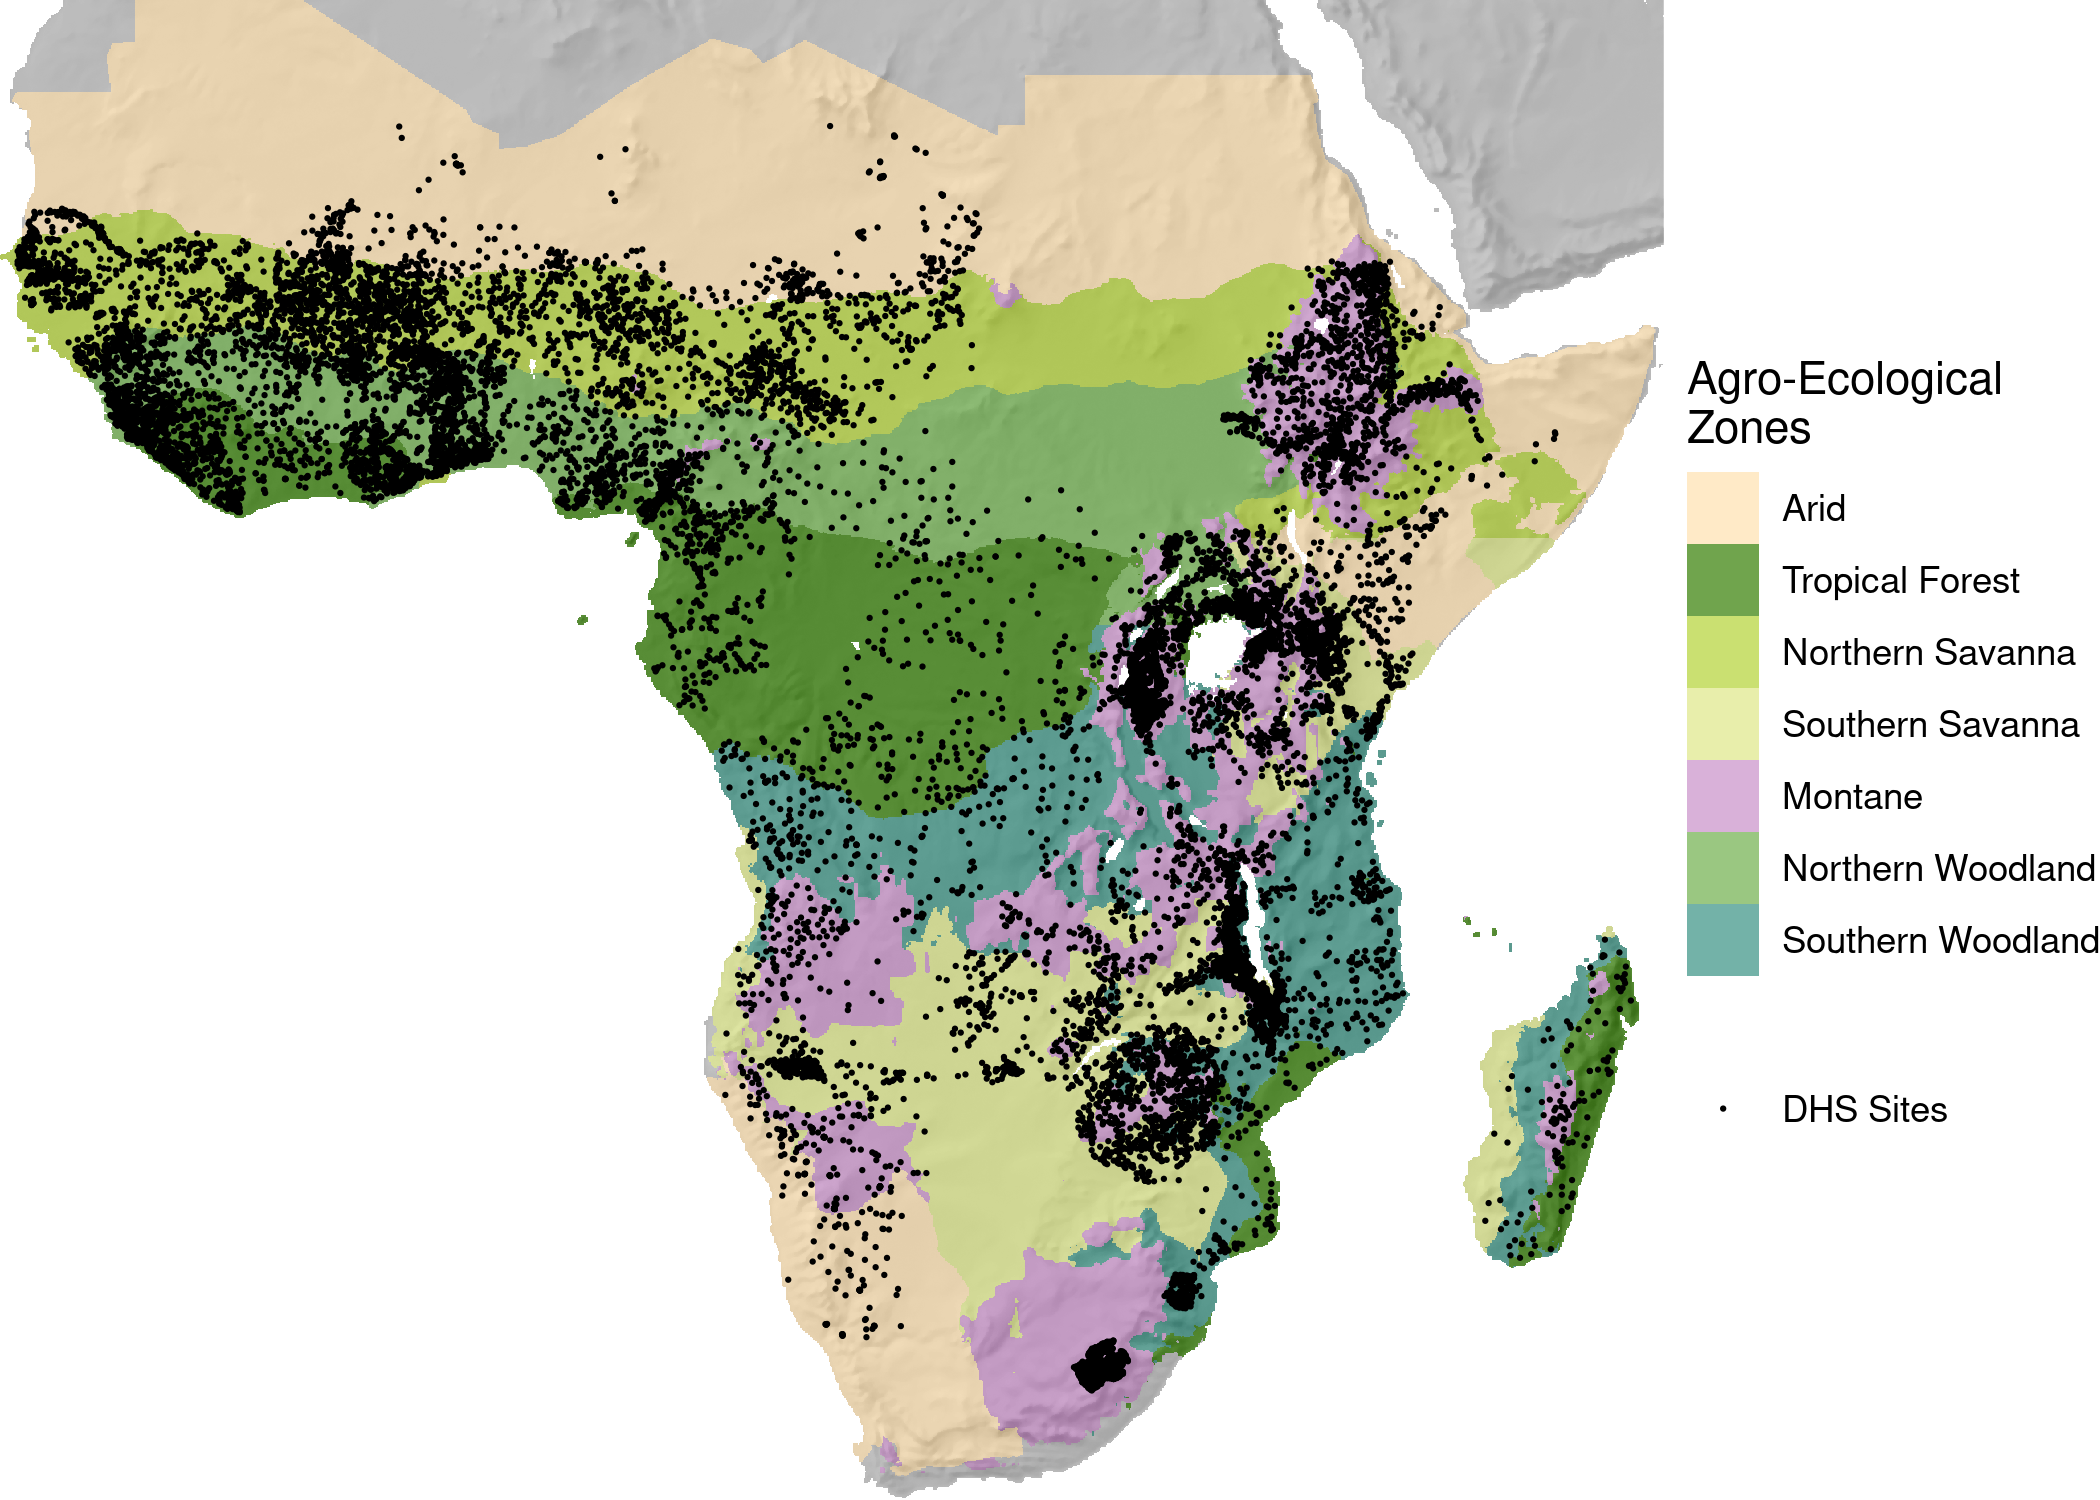
\includegraphics[width=0.8\linewidth]{AEZ_Sites.png}
	\caption{Agro-Ecological Zones and DHS sites included in the study.}
	\label{fig:AEZmap}
\end{figure}

\section{Methods}
For this analysis we model how access to ecosystem services affects the vulnerability of nutrition to drought in each agro-ecological zone.  We use a special class of Generalized Additive Model (GAM) known as a Varying-Coefficient model \cite{Wood2017} with a nonlinear smooth to model how the impact of droughts on HAZ scores varies according the amount of nearby natural land cover.  Furthermore, we use Covariate Balancing Generalized Propensity Scoring (CBGPS) to control for the effects of other geographic factors that affect drought vulnerability and may be correlated with land cover and land use, including population, subnational GDP per capita, access to larger cities, international trade.

\subsection{Covariate Balancing Generalized Propensity Scoring}
A number of factors are associated with the presence or absence of uncultivated land cover that also affect drought vulnerability.  Thus, to be able to infer that it is uncultivated land and the ecosystem services it provides that is having a causal effect on reducing drought vulnerability, it is important to control for these variables.  Propensity score weighting is a popular method to deal with this issue; however, most traditional methods involve a binary treatment variable, which must be dichotomized if it is initially measured in continuous terms \cite{Hirano2003, Robins2000}.  Because our treatment variable, uncultivated land, is continuous, and we have no theoretical priors on how it could be dichotomized, we opt instead to use Covariate Balancing Generalized Propensity Scoring (CBGPS), which can be used for continuous treatments and is more robust to mis-specification \cite{Fong2018}.  Moreover, we use the non-parametric method to estimate the generalized propensity score, which finds weights that leave each co-founding variable uncorrelated with the treatment variable, while maximizing the empirical likelihood of observing the data.  The non-parametric approach makes it possible to avoid assumptions about the functional form of the propensity score, but is more computationally costly \cite{Fong2018}.

We balance for demographic and economic factors that can influence both drought vulnerability as well as land cover.  These are: population, from the WorldPop project \cite{Tatem2017}, which can affect land cover by increasing pressure for agricultural production, as well as drought vulnerability by increasing access to off-farm labor opportunities but also increasing pressure for resources; subnational GDP per capita \cite{Kummu2018}, which can drive agricultural expansion, while also decreasing drought resilience through financial capital; national imports per capita \cite{WorldBank2017}, which can drive agricultural expansion \cite{Meyfroidt2013} while also increasing food access, even when local food production is low; and time to travel distance to major cities \cite{Weiss2018, Uchida2008}, which is an indicator of both market pressure on agriculture as well as access to financial capital that can buffer child nutrition from the effects of droughts.

After using the non-parametric CBGPS methodology to generate weights for each of these variables with respect to the availability of uncultivated land, we tested to see whether the correlation between these variables and uncultivated land cover decreased \cite{Fong2018}.  We run the algorithm separately for each AEZ in our analysis.  To conduct the balancing we use the CBPS package for R \cite{Fong2018a}, with the default value of $0.1/N$ for the tuning parameter $\rho$, which moderates the trade-off between completely reducing correlation and avoiding extreme outlier weights.

\subsection{Modeling Framework}
Having derived weights for the propensity of each observation to have uncultivated land in its vicinity, we then model nutrition outcomes as a function of the local 24-month SPEI score, where the coefficient for SPEI is modeled as a function of uncultivated land cover, controlling for typical household and individual factors as well as the spatially-varying rate of malnutrition using a spherical spline.  This is a specific form of Generalized Additive Model \cite{Hastie1986} known as a varying coefficient model \cite{Wood2017}.  Specifically, or model takes the following form:

\begin{equation}
 y = \beta_0 + \beta X + s(latitude, longitude) + s(\nu) spei + \epsilon \label{eqn:GAM}
\end{equation}

Where $y$ is a given child's HAZ score, $\beta_0$ is a fixed intercept, $X$ is a matrix of individual and household covariates, modified by a vector of fixed coefficients $\beta$, $s(latitude, longitude)$ is a spatially varying effect estimated by a spherical spline basis \cite{Wahba1982}, and $s(\nu)$ is a coefficient for the effect of the 24-month SPEI on nutrition outcomes, with the coefficient varying as a function of uncultivated land cover $\nu$, and with each function $s(\nu)$ estimated separately for each AEZ.  The basis we use for the varying coefficient $s(\nu)$ is estimated using thin plate splines \cite{Duchon1977}, and the smoothing parameter for this smooth is estimated through Generalized Cross Validation (GCV) \cite{Wood2017}.

\subsection{Modeling Contribution of Uncultivated Land to Drought-Resilient Nutrition}
To estimate the contribution of uncultivated land to nutrition outcomes, we model two scenarios for every AEZ where natural land cover was found to buffer children from the effects of drought: one estimating the impact of drought on child HAZ scores based on current levels of natural land cover, and one counterfactual scenario estimating the impact of drought on child HAZ scores if natural land cover were converted to agriculture.

Our model estimates changes in mean HAZ scores under drought conditions, but not increases in rates of stunting, which is a more familiar metric for policymakers. Given that HAZ scores are normally distributed and the rate of stunting is the percentage of children under 5 years old with an HAZ score of less than -2, it is possible to covert changes in mean HAZ scores into increases in rates stunting given prevailing mean HAZ scores, which can in turn be derived from prevailing rates of stunting and the standard deviation of HAZ scores.  Thus, for estimates of current HAZ scores, we use data from a recent analysis of rates of stunting in Africa \cite{Osgood-Zimmerman2018}.  Because this analysis estimated rates of stunting for the years 2000-2015, we draw on trend analysis methods common in epidemiology to conduct a pixel-wise forecast to the year 2020 \cite{Fullman2017, Osgood-Zimmerman2018}.  For standard deviation, overall standard deviations in HAZ scores have been observed to vary independently of mean HAZ scores \cite{Mei2007} and to not change significantly over time.  Thus, we simply use the standard deviation for our dataset (1.62), which matches previous literature on the standard deviation of HAZ scores in surveys in Africa \cite{Mei2007}.

Using these values and the definition of a normal distribution, we estimate the current HAZ scores as well as the decrease in HAZ scores under drought for scenarios of natural land cover as well as a counterfactual scenario with no natural land cover.  Then we derive a pixelwise estimate of increases in rates of stunting under drought in the absence of natural land cover providing ecosystem services.

\section{Results}
\subsection{Covariate Balancing}
After estimating weights using CBGPS, the correlation between uncultivated land cover and the various confounding variables that we attempted to control for was significantly reduced.  Tables \ref{tab:CBPSsum1} and \ref{tab:CBPSsum2} show the reduction in correlation between these variables based on the weighting.

\begin{table}[h!]
	\begin{center}
		\begin{tabular}{r | c c c c c c c c }
	&	\multicolumn{2}{c}{Import Value Per Capita}			&	\multicolumn{2}{c}{Population Density}			\\
	\cmidrule(lr){2-3}\cmidrule(lr){4-5}
AEZ	&	Unweighted	&	Weighted	&	Unweighted	&	Weighted	\\
\hline									
Arid	&	0.22	&	0.01	&	0.27	&	0	\\
Forest	&	0.1	&	0.1	&	-0.47	&	0.04	\\
Highlands	&	0.37	&	0.03	&	-0.64	&	-0.14	\\
Northern Savanna	&	0.02	&	0.03	&	-0.45	&	0.02	\\
Northern Sub-Forest	&	0.16	&	-0.03	&	-0.41	&	-0.01	\\
Southern Savanna	&	0.45	&	0.01	&	-0.62	&	-0.03	\\
Southern Sub-Forest	&	0.46	&	-0.09	&	-0.7	&	0.18	\\	
		\end{tabular}
	\caption{Summary of correlation between uncultivated land cover and confounding variables before and after weighting using CBGPS}
	\label{tab:CBPSsum1}
	\end{center}
\end{table}

\begin{table}[h!]
	\begin{center}
		\begin{tabular}{r | c c c c c c c c }
			\cmidrule(lr){2-3}\cmidrule(lr){4-5}
	&	\multicolumn{2}{c}{Subnational GDP Per Capita}			&	\multicolumn{2}{c}{Time to Travel to Major City}			\\
	\cmidrule(lr){2-3}\cmidrule(lr){4-5}
AEZ	&	Unweighted	&	Weighted	&	Unweighted	&	Weighted	\\
\hline									
Arid	&	0.16	&	-0.01	&	-0.15	&	0	\\
Forest	&	0.19	&	0.08	&	0.31	&	-0.03	\\
Highlands	&	0.17	&	-0.04	&	0.33	&	0.12	\\
Northern Savanna	&	-0.16	&	0.02	&	0.24	&	0.01	\\
Northern Sub-Forest	&	-0.03	&	-0.04	&	0.12	&	0.03	\\
Southern Savanna	&	0.47	&	0.02	&	0.24	&	0.05	\\
Southern Sub-Forest	&	0.22	&	0.06	&	0.17	&	0.05	\\
\end{tabular}
\caption{Summary of correlation between uncultivated land cover and confounding variables before and after weighting using CBGPS}
\label{tab:CBPSsum2}
\end{center}
\end{table}


\subsection{Role of Natural Land Cover in Moderating Drought by AEZ}

Having estimated the model, our main parameters of interest are the smooths for how uncultivated land cover affects the impact of drought in each AEZ.  Thus, we graph those effects here in Figure \ref{fig:naturaleffect}, and include full model results in the Appendix.

\begin{figure}[h!]
	\begin{center}
	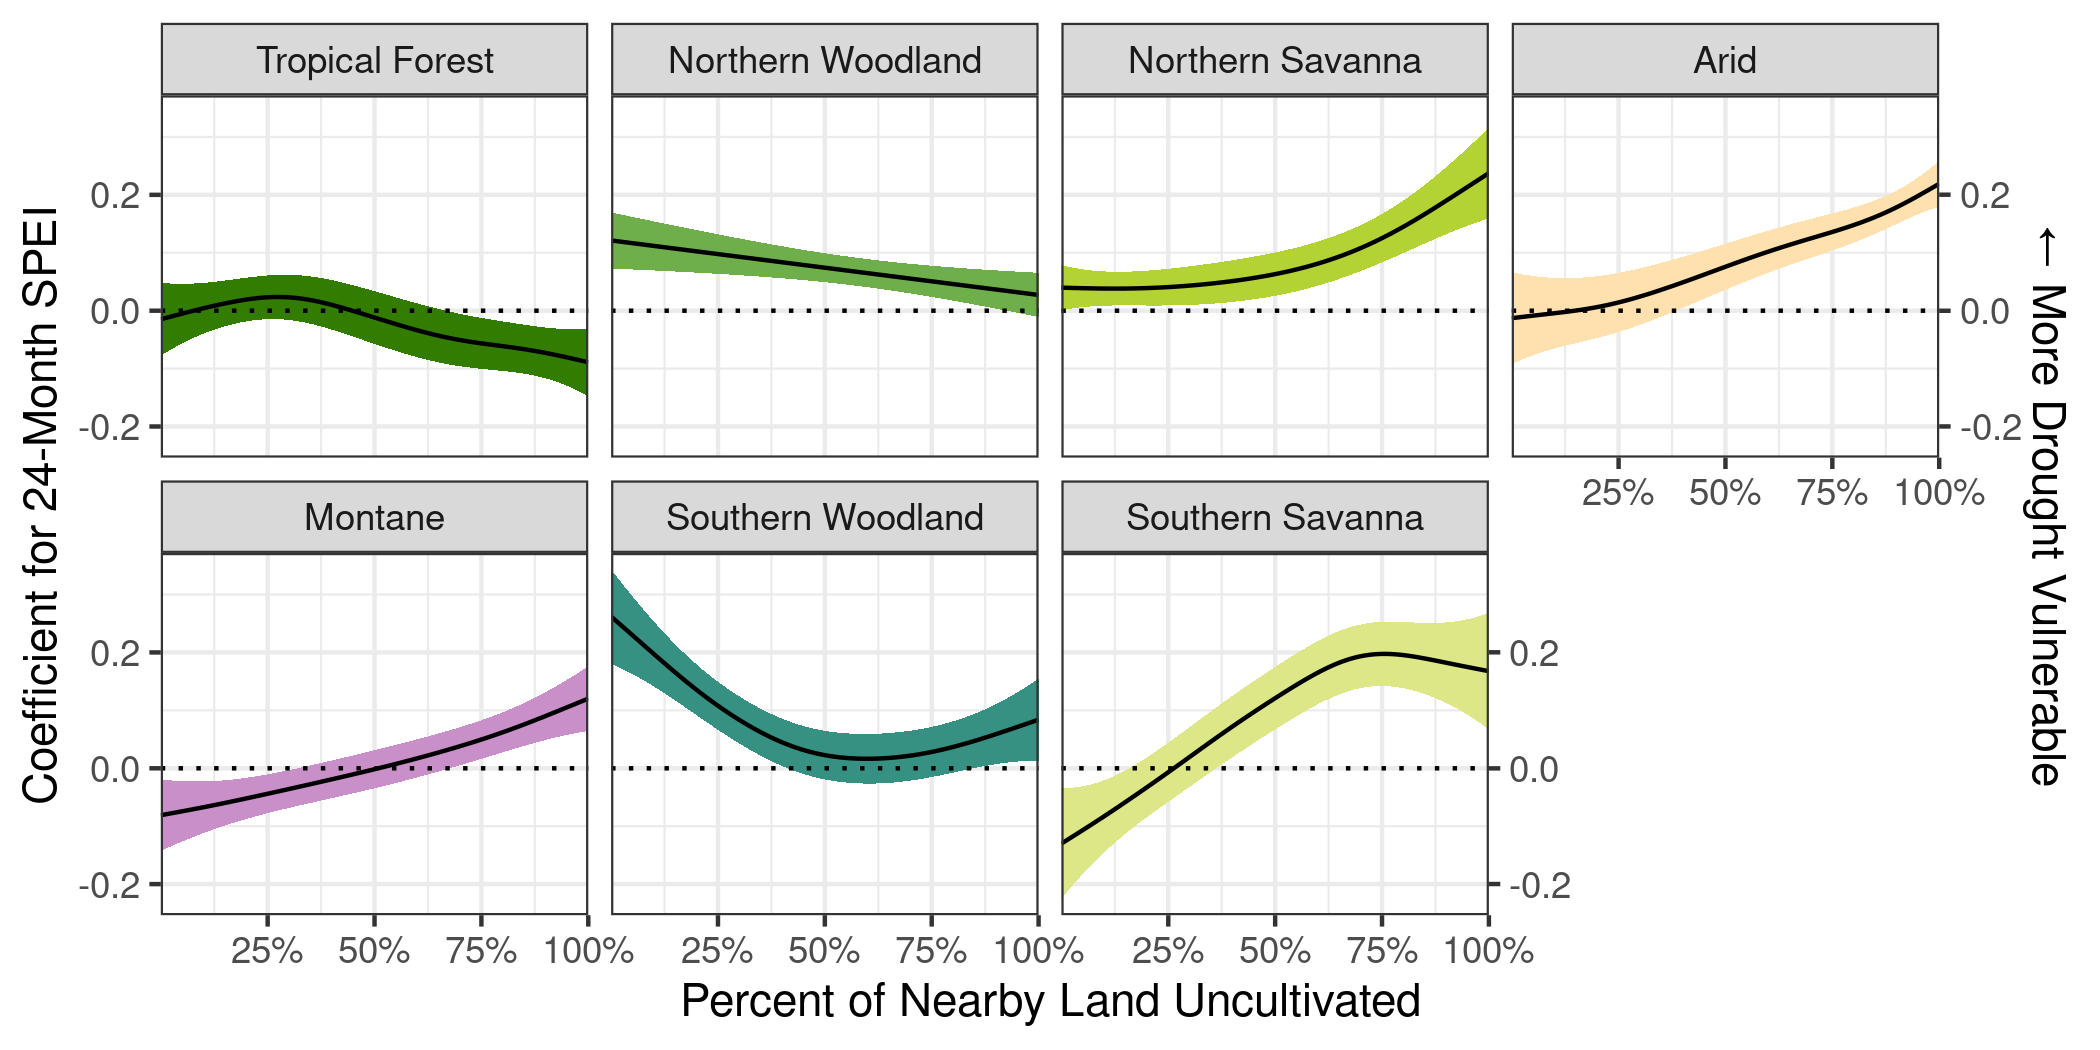
\includegraphics[width=0.8\linewidth]{AEZ_effects.png}
	\end{center}
	\caption{Varying effect of droughts on child nutrition outcomes by Agro-Ecological Zone (AEZ).  In arid, savanna, and highland zones, more natural land cover was associated with greater drought vulnerability, while in sub-forest zone, natural land cover was associated with less drought vulnerability.  Error bands indicate the 95\% confidence interval.}
	\label{fig:naturaleffect}
\end{figure}

Figure \ref{fig:naturaleffect} shows how the coefficient for the 24-month SPEI varies as a function of the percent of nearby natural land cover.  The error band around the parameter indicates the 95\% confidence interval.  Thus, areas where the error band does not cross 0 (at the dotted line) indicates that, at that level of natural land cover, precipitation anomalies have a significant effect on child nutrition outcomes.

In many AEZs, increasing rates of natural land cover are modeled to have a higher coefficient for the 24-month SPEI, signaling greater drought vulnerability.  However, in the sub-forest AEZ of both northern and southern Africa, decreasing natural land cover is associated with greater drought vulnerability.  At low levels of natural land cover in both northern and southern sub-forest africa, a moderate drought (SPEI = -2) decreases mean HAZ scores by 0.2 to 0.4, whereas at high levels of natural land cover, drought has no significant effect on nutrition outcomes.

\subsection{Modeling Ecosystem Service Dependence Over Space}
Our model indicates that in sub-forest parts of Africa, natural land cover buffers child nutrition from the effects of drought.  Thus, focusing on these AEZs, we model the impact of drought on child nutrition outcomes in scenarios of both current natural land cover levels as well as with no natural land cover, and estimate potential increases in stunting.

\begin{figure}[h!]
	\begin{center}
		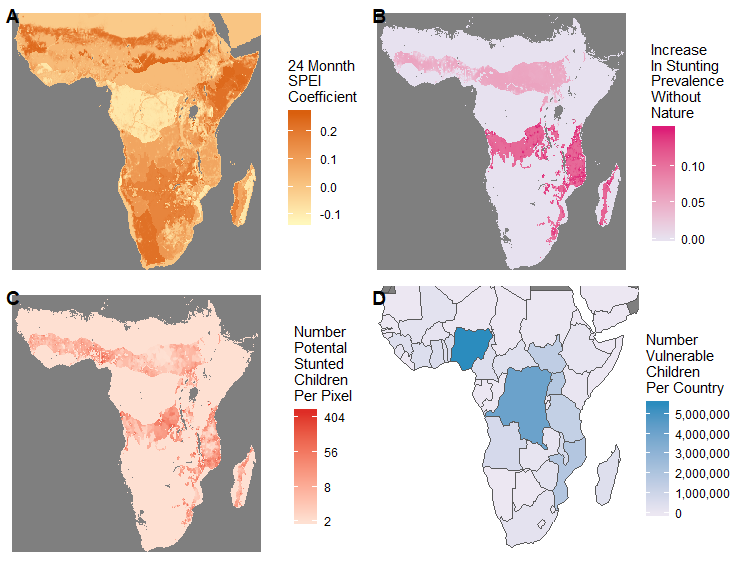
\includegraphics[width=0.8\linewidth]{AfricaEffects.png}
		\caption{\textbf{A}) The effects of the 24-month SPEI on HAZ scores across Africa.  Positive values indicate drought vulnerability. \textbf{B}) Increase in the rate of stunting under drought if local uncultivated land were entirely converted to agriculture.  \textbf{C}) The gross number of additional stunted children per pixel in a no natural land cover scenario. \textbf{D}) The number of children dependent on local natural land cover for drought resilience by country, including those that wouldn't necessarily become stunted.}
		\label{fig:AfricaEffects.png}
	\end{center}
\end{figure}

Figure \ref{fig:AfricaEffects.png} shows several outputs from the steps from extrapolating the parameters from our model to estimating the total number of children dependent on local ecosystem services for drought resilience per country.  The most drought vulnerable areas are arid and savanna AEZs, especially in the Sahel, the Horn of Africa, as well as in arid parts of Southwest Africa.  However, the areas that would see an increase in stunting in the absence of local natural land cover were mostly in the sub-forest regions on Northern and Southern Africa, such as the Guinean forest-savanna mosaic of Northern and Western Africa as well as the Miombo Woodlands of Southern Africa. Examining the potential increase in stunted child under drought in each of these eco-regions shows that many of them would be located in the woodlands of southern DRC and northern Angola, as well as in parts of Mozambique and southern Tanzania.  Throughout Africa, an additional 1.5 million children would be stunted under drought without local ecosystem services.  Finally, examining the total number of vulnerable children, which would see any decrease in HAZ scores without necessarily becoming stunted without local ecosystem services shows that they are predominantly in the countries of Nigeria and DRC.

\section{Discussion}

This paper assessed how the prevalence of uncultivated land cover moderated the impact of drought on child nutrition outcomes throughout several agro-ecological zones in Africa.  We took care to control for the potential confounding effects of several factors that could influence both the presence of uncultivated land as well as drought vulnerability, such as GDP per capita, distance to major cities, population density, and the per capita value of national imports.  We found that the manner in which natural land cover moderated the effect of drought on child nutrition outcomes varied by AEZ, and that there is an observable ``safety net" effect in semi-forested landscapes throughout Africa, although natural land cover is associated with greater drought vulnerability in arid and savanna AEZs.  Finally, examining a counterfactual scenario of the impact of droughts without uncultivated land cover and the ecosystem services it provides shows that millions of children are dependent on ecosystem services to meet their nutrition needs in times of drought.

A major contribution of this paper to the literature is its scale.  Most other studies of the role in ecosystem services in buffering human well-being from climate shocks tends to focus on case studies \cite{Debela2012} as well as use hypothetical scenarios \cite{Robledo2012} or retrospective analyses \cite{Muller2008}.  This paper provides a large scale analysis of nutrition outcomes observed during varying levels of drought as well as across sites with varying access to ecosystem services.

One of the only multinational analyses of the role of ecosystem services as a buffer during shocks found that households didn not rank forest resources as a very important resource during shocks \cite{Wunder2014}.  This paper differed in significant ways from our analysis: it focused on forests rather than all uncultivated land cover types, it focused on a variety of types of shocks beyond just drought, it asked households retrospectively about previous shocks rather than observing them \textit{in situ}, and it asked households about their preferences.  Thus, there are several reasons why we observed natural land cover as playing as significant effect in buffering households from drought in semi-forested landscapes while Wunder et al. did not find such an effect.  Firstly, it may be that households do not pivot towards forest resourced during drought; rather, households that are always using forest resources are simply less affected by agricultural shocks like drought.  Secondly, by focusing only on forest resources like timber, Wunder et al. are unable to explore the benefit that supporting and regulating ecosystem services have on local agricultural production.  

An important aspect of this analysis was using weighting to ameliorate the effects of potential confounding variables.  Because we controlled for the effects of several demographic and economic variables, we can more confidently ascribe the observed drought mitigation to the land cover itself rather than to another factor that is correlated with land cover.  However, given that weighting each covariate to achieve a correlation of perfectly 0 would be either impossible or would require extreme weights, we did not reduce the correlation between our confounding variables and natural land cover all the way to 0 (See Tables \ref{tab:CBPSsum1} and \ref{tab:CBPSsum2}).  Nevertheless, we diminished the correlation to the extent that a causal interpretation of the observed mitigation effect of natural land cover is now more plausible.  This, combined with the fact that we excluded households with greater than 1\% urban land cover and greater than 5\% water land cover means that we are making the best apples-to-apples comparison we can.

While the model estimated the moderating effect of natural land cover on drought vulnerability as varying across AEZs, we found that natural land cover played a similar function in ecologically similar zones.  In arid and savanna zones, greater natural land cover was associated with greater drought vulnerability.  On the other hand, in the ecological similar but geographically disjoint semi-forested regions, natural land cover had a safety net effect during drought.  The fact that ecologically similar eco-regions were modeled as having similar effects in terms of drought vulnerability, even though they were modeled with independently estimated smoothing splines, suggests that this effect is real and is ecologically based.

One potential interpretation of these findings is that ecosystem services are less valuable to livelihoods in arid and savanna environments.  This could be due to lower overall biomass leading to a decreased availability of provisioning ecosystem services: the amount of edible biodiversity is lower in very arid ecosystems compared to more lush ecosystems.  Similarly, many regulating and supporting ecosystem services provided by natural land cover, such as wind breaking, shading and temperature regulation, and moisture retention are specifically a function of trees \cite{Reed2016}. Thus, areas lacking in trees and biodiversity may not be able to provide the safety net effect that more forested areas have.  For very humid and mesic areas, other the other hand, drought vulnerability does not seem to be a major issue: even precipitation is well below historic norms, it is still high enough to support food production.  This may be why there was almost no effect of SPEI in the forest AEZ.  Thus, the semi-forested parts of Africa present a middle ground, where rainfall levels are low enough that a precipitation anomaly can lead to increases in stunting, but rainfall is still high enough that natural land cover has both the biodiversity and biomass to provide a safety net.

While the association between natural land cover and reduced drought vulnerability in certain AEZs is certainly suggestive that people are relying on ecosystem services as a safety net, this analysis cannot speak to the particular pathways through which people are benefiting from nature.  For example, the relative importance of provisioning ecosystem services such as wild foods versus regulating services such as shading to prevent moisture loss cannot be ascertained.  Nevertheless, previous work in Africa has found that greater natural land cover is associated with greater collection of wild foods and nonfood NTFPs, suggesting that provisioning ecosystem services are a part of the pathway \cite{Cooper2018a}.

\section{Conclusion}
These findings are have important implications for the study of food security, climate change vulnerability, and environmental conservation.  We showed that nature can be a critical part of reducing climate change vulnerability, but the specific role that nature plays is highly context-specific.  While mapping ecosystem services has traditionally focused on variables like carbon stocks and biodiversity hotspots, this analysis shows that the contributions of nature to food security can also be mapped to support greater food security.  Given the increasing threat of a more drought prone world under climate change \cite{Dai2013} combined with the severe precarity of Africa's agrarian poor, dampening the effects of drought and providing alternative food and income sources when agriculture fails may indeed be one of nature's most important contributions to people.


\bibliographystyle{apalike}
\bibliography{C://Users/matt/library}

\setcounter{section}{0}
\renewcommand{\thetable}{A\arabic{section}}
\section*{Appendix} \label{AppendixA}
\setcounter{table}{0}
\setcounter{figure}{0}
\renewcommand{\thetable}{A\arabic{table}}
\renewcommand{\thefigure}{A\arabic{figure}}



\begin{longtable}{l c }
\hline
 &  \\
\hline
\endfirsthead
\hline
 &  \\
\hline
\endhead
\hline
\endfoot
\hline
\multicolumn{2}{l}{\scriptsize{$^{***}p<0.001$, $^{**}p<0.01$, $^*p<0.05$}}\\
\caption{Statistical models}
\label{table:coefficients}
\endlastfoot
age                              & $-0.02^{***}$  \\
                                 & $(0.00)$       \\
birth\_order                     & $0.01^{***}$   \\
                                 & $(0.00)$       \\
hhsize                           & $-0.00$        \\
                                 & $(0.00)$       \\
sexFemale                        & $-17.07^{***}$ \\
                                 & $(1.44)$       \\
sexMale                          & $-17.19^{***}$ \\
                                 & $(1.44)$       \\
mother\_years\_ed                & $0.03^{***}$   \\
                                 & $(0.00)$       \\
toiletNo Facility                & $-0.16^{***}$  \\
                                 & $(0.01)$       \\
toiletOther                      & $-0.14^{***}$  \\
                                 & $(0.03)$       \\
toiletPit Latrine                & $-0.13^{***}$  \\
                                 & $(0.01)$       \\
interview\_year                  & $0.01^{***}$   \\
                                 & $(0.00)$       \\
as.factor(calc\_birthmonth)2     & $-0.02$        \\
                                 & $(0.02)$       \\
as.factor(calc\_birthmonth)3     & $0.04^{*}$     \\
                                 & $(0.02)$       \\
as.factor(calc\_birthmonth)4     & $0.03^{*}$     \\
                                 & $(0.02)$       \\
as.factor(calc\_birthmonth)5     & $0.03^{*}$     \\
                                 & $(0.02)$       \\
as.factor(calc\_birthmonth)6     & $0.15^{***}$   \\
                                 & $(0.02)$       \\
as.factor(calc\_birthmonth)7     & $0.11^{***}$   \\
                                 & $(0.02)$       \\
as.factor(calc\_birthmonth)8     & $0.18^{***}$   \\
                                 & $(0.02)$       \\
as.factor(calc\_birthmonth)9     & $0.17^{***}$   \\
                                 & $(0.02)$       \\
as.factor(calc\_birthmonth)10    & $0.23^{***}$   \\
                                 & $(0.02)$       \\
as.factor(calc\_birthmonth)11    & $0.23^{***}$   \\
                                 & $(0.02)$       \\
as.factor(calc\_birthmonth)12    & $0.44^{***}$   \\
                                 & $(0.02)$       \\
head\_age                        & $0.00^{***}$   \\
                                 & $(0.00)$       \\
head\_sexMale                    & $-0.07^{***}$  \\
                                 & $(0.01)$       \\
wealth\_norm                     & $0.54^{***}$   \\
                                 & $(0.02)$       \\
AEZ\_newafr.forest.4             & $-0.11^{***}$  \\
                                 & $(0.03)$       \\
AEZ\_newafr.high.7               & $-0.22^{***}$  \\
                                 & $(0.03)$       \\
AEZ\_newnafr.sav.5               & $0.00$         \\
                                 & $(0.02)$       \\
AEZ\_newnafr.subforest.8         & $0.03$         \\
                                 & $(0.03)$       \\
AEZ\_newsafr.subforest.9         & $0.06^{*}$     \\
                                 & $(0.03)$       \\
AEZ\_newseafr.sav.6              & $-0.17^{***}$  \\
                                 & $(0.03)$       \\
EDF: s(latitude,longitude)       & $45.17^{***}$  \\
                                 & $(49.00)$      \\
EDF: s(natural):afr.arid.123     & $3.24^{***}$   \\
                                 & $(3.74)$       \\
EDF: s(natural):afr.forest.4     & $3.20^{**}$    \\
                                 & $(3.74)$       \\
EDF: s(natural):nafr.sav.5       & $2.73^{***}$   \\
                                 & $(3.16)$       \\
EDF: s(natural):seafr.sav.6      & $3.20^{***}$   \\
                                 & $(3.75)$       \\
EDF: s(natural):afr.high.7       & $2.76^{***}$   \\
                                 & $(3.20)$       \\
EDF: s(natural):nafr.subforest.8 & $2.00^{***}$   \\
                                 & $(2.00)$       \\
EDF: s(natural):safr.subforest.9 & $2.97^{***}$   \\
                                 & $(3.46)$       \\
\hline
AIC                              & 890428.85      \\
BIC                              & 891421.48      \\
Log Likelihood                   & -445118.15     \\
Deviance                         & 16.37          \\
Deviance explained               & 0.48           \\
Dispersion                       & 0.00           \\
R$^2$                            & 0.11           \\
GCV score                        & 0.00           \\
Num. obs.                        & 221885         \\
Num. smooth terms                & 8              \\
\end{longtable}



\end{document}
